\newpage
\section{Parallelization}
\label{sec:parallelization}

\noindent
\begin{minipage}[t]{0.47\textwidth} % Colonna sinistra
    %\centering

    Ciclo \texttt{for} parallelizzato con OpenMP utilizzando \texttt{private(n)} per rendere ogni thread indipendente

    \begin{lstlisting}[basicstyle=\ttfamily\scriptsize]
#pragma omp parallel for private(n)
for (k=0 ; k<N ; k++)
{
    double Xr_temp = 0.0;
    double Xi_temp = 0.0;

    for (n=0 ; n<N ; n++)  {
        Xr_temp += ...
        Xi_temp += ...
    }

    Xr_o[k] = Xr_temp;
    Xi_o[k] = Xi_temp;
}
    \end{lstlisting}
    
    \vspace*{0.7cm}

    \centerline{\textbf{Execution time}}
    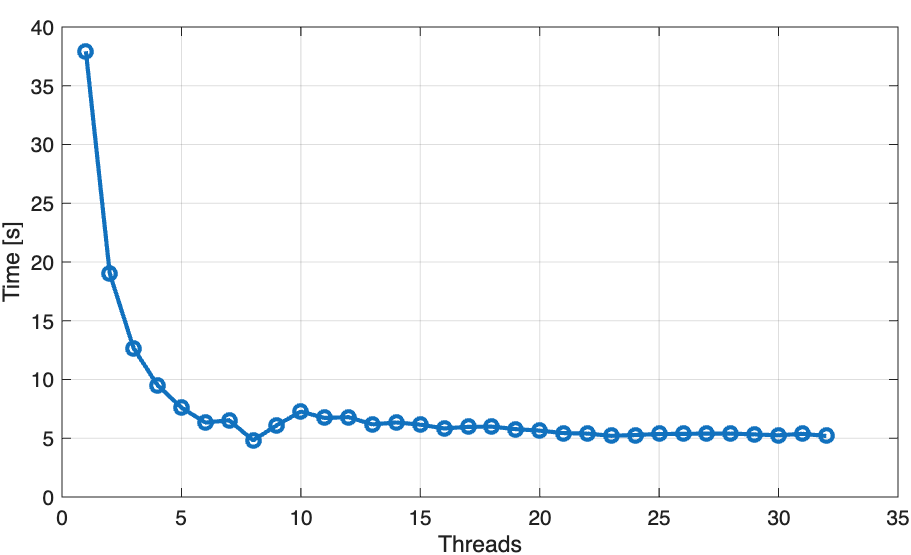
\includegraphics[width=\linewidth]{assets/parallelization/omp1_times.png}

    \vspace{0.5cm}

    \centerline{\textbf{Speedup}}
    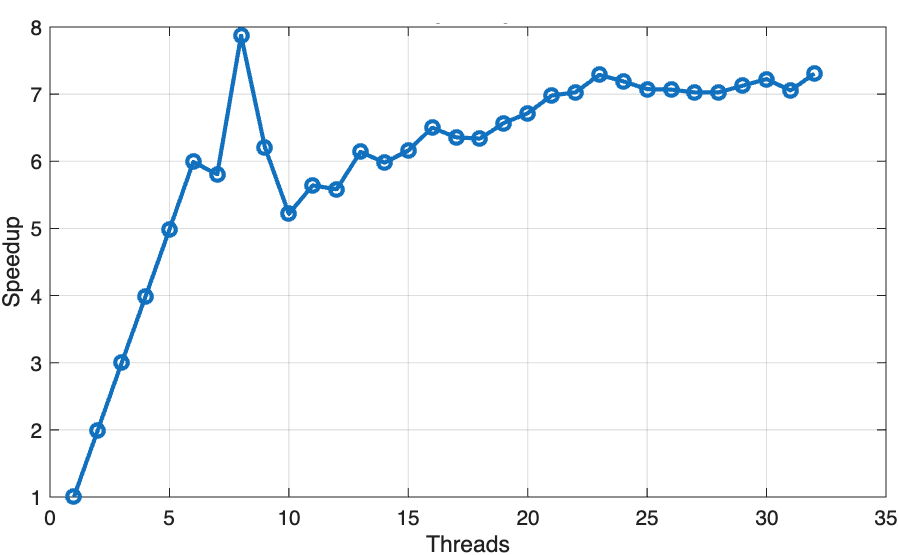
\includegraphics[width=\linewidth]{assets/parallelization/omp1_speedups.png}
    
    \vspace{0.5cm}
    
    \centerline{\textbf{Efficiency}}
    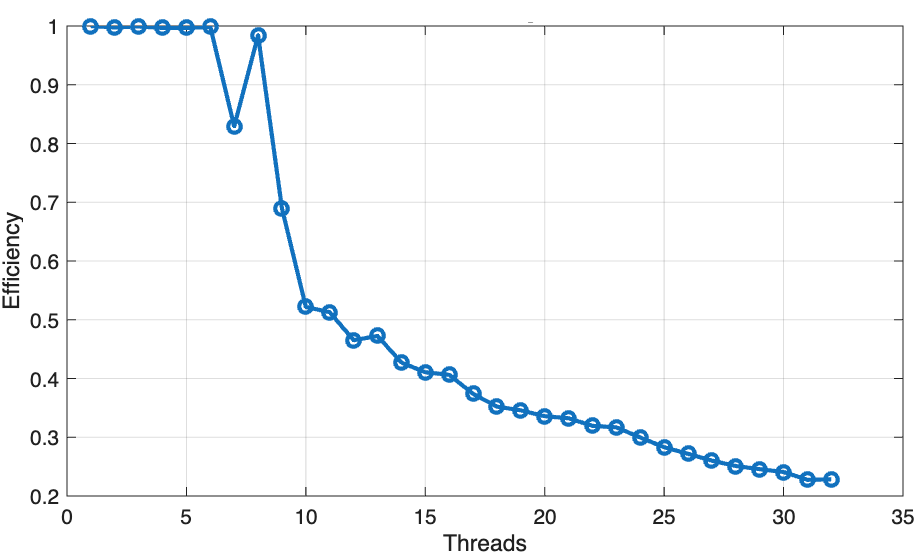
\includegraphics[width=\linewidth]{assets/parallelization/omp1_efficiencies.png}
    
\end{minipage}
\hfill
\begin{minipage}[t]{0.47\textwidth} % Colonna destra
    %\centering

    Ciclo \texttt{for} parallelizzato con OpenMP usando \texttt{reduction} per combinare i risultati dei thread.

    \begin{lstlisting}[basicstyle=\ttfamily\scriptsize]   
int k, n;
for (k=0 ; k<N ; k++)
{
    double Xr_temp = 0.0;
    double Xi_temp = 0.0;

#pragma omp parallel for reduction(+:Xr_temp, Xi_temp)    
    for (n=0 ; n<N ; n++)  {
        Xr_temp += ...
        Xi_temp += ...
    }

Xr_o[k] = Xr_temp;
Xi_o[k] = Xi_temp;
}
    \end{lstlisting}

    \centerline{\textbf{Execution time}}
    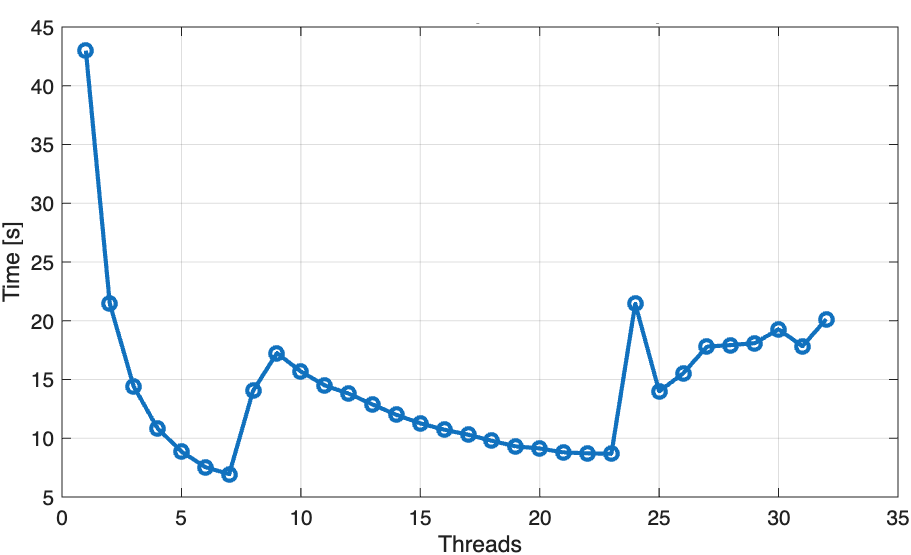
\includegraphics[width=\linewidth]{assets/parallelization/omp2_times.png}

    \vspace{0.5cm}

    \centerline{\textbf{Speedup}}
    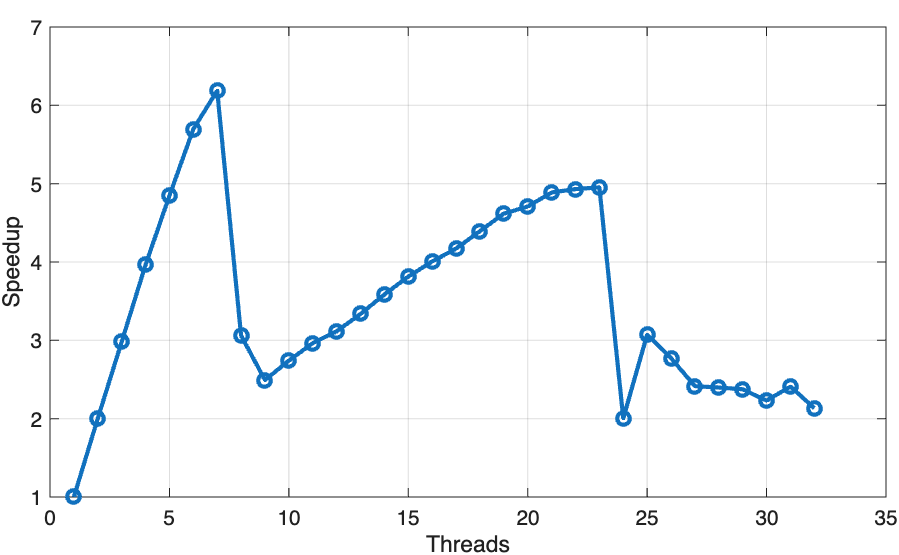
\includegraphics[width=\linewidth]{assets/parallelization/omp2_speedups.png}
    
    \vspace{0.5cm}
    
    \centerline{\textbf{Efficiency}}
    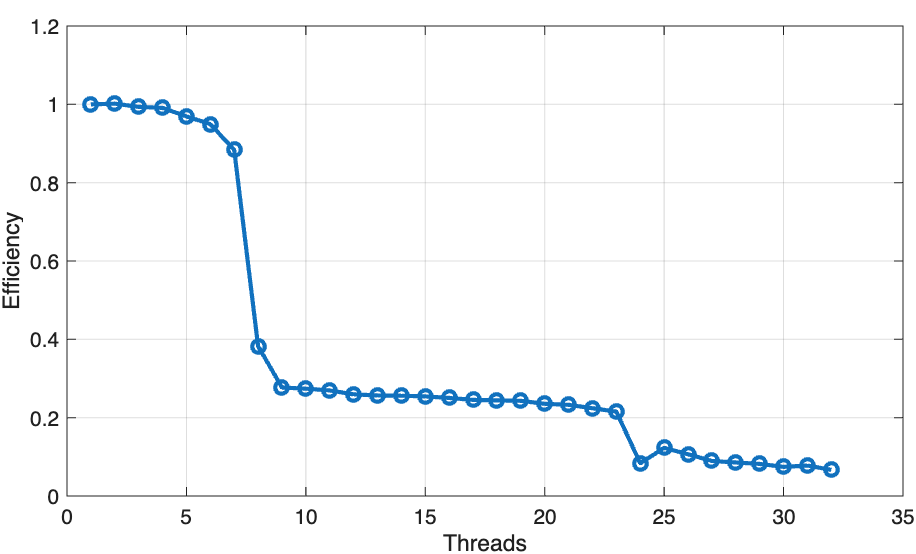
\includegraphics[width=\linewidth]{assets/parallelization/omp2_efficiencies.png}
\end{minipage}
